\section{Validation and Verification}
\subsection{Software in the loop}
The validate the IMU driver, we develop a second application that will simulate the IMU device by sending fake measurements on a virtual serial device.
The test procedure for the IMU driver is as follow:
\begin{itemize}
    \item The tester allocate two device files to simulate virtual serial port.
    \item The tester starts the software in the loop application. The application immediately starts to write fake imu measurements data to the virtual device file.
    \item The tester starts the application that contains the driver. The driver application reads data from the virtual device file.
    \item The test application displays the received data on the terminal.
\end{itemize}



\begin{figure}[ht]
    \centering
    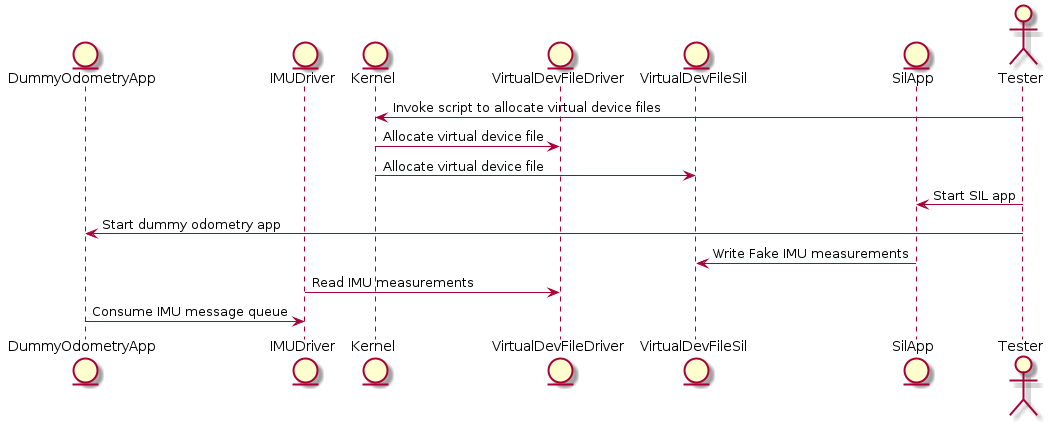
\includegraphics[width=0.75 \textwidth]{diagrams/software_in_the_loop.png}
    \caption{High level overview of SIL test procedure}
    \label{reference}
\end{figure}
